\chapter{Raw notes (To be rewritten)}

\chapter{Lecture 30/10/2025}

Modern Catalogues

Bautz-Morgan: 

sovraddensity of galaxies

Color magnitude diagram

\dots

\begin{itemize}
    \item sovraddensity of galaxies
    \item color magnitude diagram
\end{itemize}

\dots

Max BCG catalog (SDSS survey):

This catalog is 90\% pure and 85\% complete. $M \ge 10^{14} M_{\odot}$

\begin{itemize}
    \item red sequence
    \item dominant central galaxy
    \item radial profile of galaxies distribution
\end{itemize}

\subsection{Groups}

\begin{itemize}
\item \textbf{Loose Groups}

They are the most common type of groups, they include almost the 50\% of the galaxies.

\item \textbf{Compact Groups}

They are very rare.

This is the case where we have a high density of galaxies, and they are all close to each other.

$$
t_{dyn} \sim \dfrac{R}{\sigma_v} \sim 0.02 H_0^{-1}
$$

\item \textbf{Fossil Groups}

$$
\Delta m_{12} \ge 2 mag
$$

\begin{tipsblock}[Fossil Groups]
The name fossil depends of the fact that a researcher thought it was the first group ever formed in the universe.
\end{tipsblock}


% seen plots in slidespaperICL

\end{itemize}


\chapter{Lecture 04/11/2025}

\missing{Start of the lecture}

The Inter Cluster Medium (ICM) is the hot gas that fills the space between the clusters. Between 1920 and 1933 were discovered the first X-ray sources.

Telescopes:

\begin{itemize}
    \item X-ray (mono source, then extended source)
    \item UMURU
    \item Einstein
    \item Rosat
    \item Chandra
    \item XMM
    \item E-Rosat
    \item Athena
\end{itemize}

Athena to study the motion of the gas in some clusters

$$
L_X \sim 10^{43-45} erg/s
$$

FF emission: Bremsstrahlung

\begin{itemize}
    \item Groups $kT \sim 1-3 KeV$
    \item Clusters $kT \sim 10-12 KeV$ (at least $> 4-5 KeV$)
\end{itemize}



$$
E_\nu \equiv \dfrac {dL}{dV d\nu}
$$

$$
e_\nu^{ff} \propto \underbrace{n_e n_i}_{n_e^2} T^{-1/2} e ^{-\frac{h\nu}{kT}}
$$

\todo{insert plots from paper sheets A2 (right column)}

$$
E \propto \sqrt{T} n_e^2 \qquad KT \gtrsim 5 KeV
$$

ff+bf+bb:
$$
E \propto T^{-0.6} n_e^2 \qquad KT \le 2 KeV
$$

\textbf{Rosat} has a sensibility range of $0.1-2.4 KeV$. It is very useful to measure the mass of a cluster.

If the gas is homogeneous, we have: $\langle n_e^2 \rangle = \langle n_e \rangle^2$, but if the mass is not homogeneous, we have: $\langle n_e^2 \rangle \neq \langle n_e \rangle^2$.

From observations we can note that the gas mass is much smaller than the stellar mass: $M_gas \sim 5-10 M_{\star}$. An important indicator is the following ratio:

$$
\dfrac{M_{gas} \ (\sim 15 - 20\% M_{tot})}{M_{\star} \ (\sim 3-5\% M_{tot})}
$$

The higher is the total mass $M_{tot}$, the higher is the ratio $\dfrac{M_{gas}}{M_{\star}}$.

A conclusion is that clusters are richer in gas, while groups are richer in stars. Follows that the clusters retain better the gas, and the groups are more efficient in forming stars.

Since $e_x \propto n_e^2$, the x-ray emission comes from the core of the cluster, therefore you can have a better view of where the cluster is in space (for distances $< 1 Mpc$). There is still the problem of the flux limit.

\subsubsection{Clusters morphology}

We can find different morphologies for the clusters:

\begin{itemize}
    \item \textbf{Unimodal Clusters}: they have a single peak in the x-ray emission.
    \item \textbf{Bimodal Clusters}: they have two peaks in the x-ray emission.
\end{itemize}

We can talk further about substructures in the clusters.

\textbf{Unimodal clusters}

$\beta-model$

\begin{itemize}
    \item 3 dimensional profile:

    $$
    \rho_{gas}(r) = \rho_{0, gas} \left( 1 + \left( \dfrac{r}{\beta r_{c, gas}} \right)^2 \right)^{-\frac{3}{2} \beta_{fit, gas}}
    \qquad \Rightarrow \qquad 
    r^{-2} \beta_{fit, gas} = \dfrac 23
    $$

    \item 2 dimensional profile:
    
    $$
    \Sigma_{gas}(R) = \Sigma_{0, gas} \left( 1 + \left( \dfrac{r}{\beta R_{c, gas}} \right)^2 \right)^{-\frac{3}{2} \beta_{fit, gas} + \frac 12}
    \qquad \Rightarrow \qquad 
    R^{-1}
    $$
    
    \item observed profile:
    
    $$
    S_x = S_{x, 0} \left( 1 + \left( \dfrac{r}{\beta R_{c, gas}} \right)^2 \right)^{-3 \beta_{fit, gas} + \frac 12}
    \qquad \Rightarrow \qquad 
    S_x = \int \rho_{gas}^2
    $$
\end{itemize}

We have a typical ICM density of:
$$
n_e \sim \dfrac{1 \cdot 10^{-3}}{cm^{-3}}
$$

Cooling Flows (or, in older literature, Cool Cores) are clusters with a high density of gas in the center, characterized by a big emission in the center.

$$
t_{cool} = \dfrac {\mu}{e_ff} \sim \underline{8.5 \cdot 10^{10} yr} \left( \dfrac{n_e}{10^{-3} cm^{-3}} \right) \left( \dfrac{T_{gas}}{10^8 K} \right)
$$

Which is bigger than the Hubble time $t_H \sim 13 \cdot 10^{9} yr$, therefore we have no cooling.

$$
\omega = \dfrac 32 n_e k T
$$

$$
E^{ff} \propto n_e^2 T^{1/2}
$$

The center of some clusters can have high $n_e$ and a lower $t_{cool} < t_H$, therefore we have a cooling core. In these kind of clusters we can observe star formation from the gas.

These kind of clusters have no big Surface Brightness \dots

\missing{something about No Cool Core and Mergers}

\subsubsection{Sunyaev-Zel'dovich Effect}

% page 252 of Schneider's book

The Sunyaev-Zel'dovich Effect is a small distortion of the Cosmic Microwave Background Radiation (CMBR) due to the interaction with the ICM.

\begin{figure}[H]
    \centering
    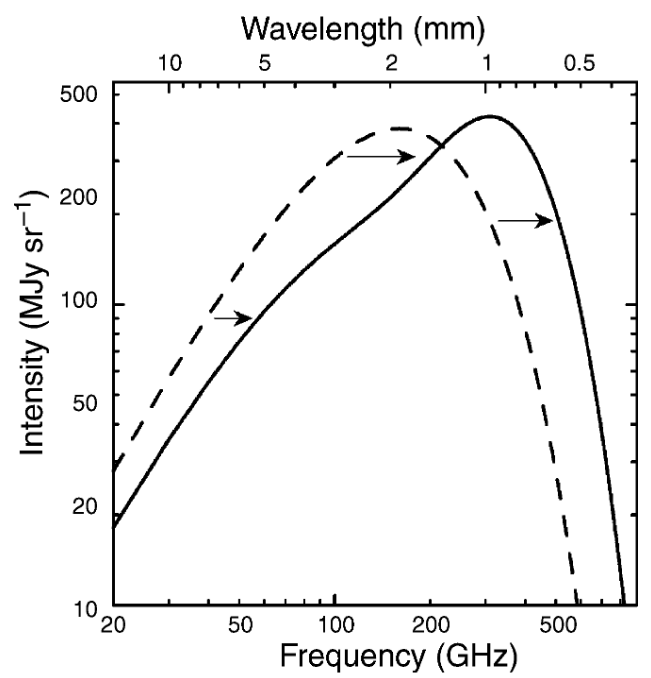
\includegraphics[width=0.4\textwidth]{assets/s-z-effect.png}
    \caption{\centering Sunyaev-Zel'dovich Effect \cite{schneider}}
\end{figure}

In the Rayleigh-Jeans domain of the CMB spectrum, thus at wavelengths larger than about 1 mm, photons are effectively removed by the SZ effect. For the change in specific intensity in the RJ part, one obtains:

$$
\dfrac {\Delta I_\nu^{RJ}} {I_\nu^{RJ}} = -2 y
$$

where $y$ is the \bfit{Compton-y parameter}:

$$
y =\int_0^\infty dl \dfrac{kT_{gas}}{m_e c^2} \sigma_T n_e
$$

and $\sigma_T$ the Thomson cross-section for electron scattering:

$$
\sigma_T = \dfrac{8 \pi}{3} \left( \dfrac{e^2}{m_e c^2} \right)^2
$$

therefore:
\begin{itemize}
    \item $y \propto$ optical depth
    \item $y \propto n_e$ 
    \item $y \propto T_{gas}$ 
\end{itemize}

So y can be a proxy for cluster mass.

$$
\theta = \dfrac R{D_A}, \quad d\theta = \dfrac{dR}{D_A}
$$
$$
sz-eff = \int d^2 \theta y = \dfrac 1{D_A^2} \int d^2 Ry \propto \dfrac 1{D_A^2} \int dV n_e T_{gas}
$$

$$
Y_{sz} \equiv M_{gas} \cdot T_{gas}
$$

\subsubsection{Radio extended emission}

There are galaxies with very large radio halos ($\sim 1 Mpc$ in size).

Radio Relics -> elongated halos, polarized light

synchrotron emission:

We have a (very weak) magnetic field $B$ (\le 1 $\mu G$) and a gamma factor $\gamma \sim 10^4$


% primary electron models (?)
For instance, if $\gamma = 300$, then the electron energy is $E = \gamma m_e c^2 \sim 150 MeV$.

But if we consider a time $T_{life} = 10^9$ its energy will be fewer and fewer.
% ???

protons instead have a shorter lifetime. 
% no from astrophysical

Bimodal clusters mergers can result in:
\begin{itemize}
    \item \textbf{Shocks}: 
    \begin{itemize} 
        \item $v_{rel} \sim 1-2 \cdot 10^3 km/s$
        \item gravitational energy: $10^64 erg$
        \item dissipation: $3 \cdot 10^63 erg$
    \end{itemize}

    \item \textbf{Turbulence}:
    \begin{itemize}
        \item ...
    \end{itemize}
\end{itemize}

\missing{last few minutes of the lecture}

\chapter{Lecture 06/11/2025}

\subsubsection{Frequencies}

VLA instruments works at a frequency of 1.4 GHz. while LOFAR has a range of 300-800 MHz.

They allow us to study phenomena such as mergers, with ratios 1:1 to 1:10.

They allow us also to study AGN and their radio emission. There are three main models:

\begin{itemize}
    \item primary electrons models: not good because it (something with the scale)
    \item primary electron reacceleration models: good because it explains the radio emission of some clusters.
    \item secondary electron reacceleration models: no evidence of it.
\end{itemize}

\subsubsection{Galaxies and X-ray emission} % schneider book page 246

Sarazin 1986-88 did a lot of studies and pubblications about the X-ray emission of galaxies.

\textbf{ICM}

We assume that the gas in the cluster is adiabatic (= isotropic)

We remember that for an ideal gas it holds that:

$$
pV = n_{mol} R T = n_{mol} \mathcal{N} \dfrac R{\mathcal R} T
$$

so we get:

$$
pV = N K_B T \qquad \Rightarrow \qquad p = \dfrac{N K_B T}{V}
$$


$$
\rho_{gas} = \rho = n \langle m \rangle = n \mu m_p
$$

we can define $\mu$ as the mean atomic mass:

$$
\mu \equiv \dfrac{\langle m \rangle}{m_p} \sim 0.6
$$

therefore, we get:

$$
\boxed{p = \rho \dfrac{K_B T}{\mu m_p}}
$$

in an isothermal situation, we have:

$$
p = k \rho
$$

And in an adiabatic situation, we have:

$$
p = k^i \rho^{\gamma}
$$

where $\gamma = \dfrac{c_p}{c_v} = \dfrac{5}{3}$ for a monatomic gas.

\textbf{Hydrostatic equilibrium}

We can observe that the cluster is in hydrostatic equilibrium:

$$
t_{sc} = \dfrac{2 R_A}{c_s},
\qquad \qquad
c_s^2 = \left.\dfrac{dp}{d\rho} \right|_{\rho = \rho_0}
$$
where $c_s$ is the sound speed:

$$
c_s \sim \sqrt {\dfrac p \rho} = \sqrt {\dfrac{n K_B T}{\mu m_p}} \sim \sqrt{1000 km/s}
$$

Therefore we observe a value of $t_sc$ smaller than the Hubble time (time of the universe):

$$
t_{sc} \sim 7 \cdot 10^8 yr < 13 \cdot 10^9 yr = t_H
$$

---

$$
\vec \nabla p = - \rho \vec \nabla \phi
$$

sphere:

$$
\dfrac {dp}{dr} = - \rho \dfrac {G M(r)}{r^2}
$$

to convince us:

$$
p = \dfrac FA \quad \Rightarrow \quad \dfrac px = \dfrac FV
$$

so 

$$
\vec \nabla p \cdot V = -m \vec \nabla \phi
\qquad \Rightarrow \qquad
\vec \nabla p = - \rho \vec \nabla \phi
$$

Coming back, we have:

$$
\dfrac{GM(r)}{r^2} =  - \dfrac 1{\rho} \dfrac{K}{\mu m_p} \left( \rho \dfrac{dT}{dr} + T \dfrac{d\rho}{dr} \right)
$$

$$
M(r) = - \dfrac 1{G} \left( \dfrac{KT}{\mu m_p} \right) r \left[ \dfrac{d \ln \rho_{gas}}{d \ln r} + \dfrac{d \ln T}{d \ln r} \right]
$$

In a 3D situation, we have:

$$
\rho_{gas}(r) = \rho_{gas, 0} \left( 1 + \left( \dfrac{r}{r_{c, gas}} \right)^2 \right)^{-\frac{3}{2} \underbrace{\beta_{fit, gas}}_{\sim 2/3}}
$$

where, if $ r \gg r_{c, gas} $, we have $\rho \to r^{-2}$.

For galaxies, we have - Jeans Equation:

$$
M(r) = - \dfrac 1{G} \sigma_r^2 r \left[ \dfrac{d \ln \rho_{gas}}{d \ln r} + \dfrac{d \ln \sigma_r^2}{d \ln r} + 2 \beta \right]
$$

Where the factor $\beta$ is called \textit{the velocity anisotropy parameter}.

$$
\beta(r) = 1 - \dfrac{\sigma_{\tau}^2}{\sigma_r^2}, 
\qquad \qquad \text{where } \ \ 
\sigma_{\tau}^2 = \dfrac {\sigma_{\theta}^2 + \sigma_{\phi}^2}2
$$

for an isotropic orbit, gas is a collisional component, therefore we have:

$$
\boxed{\beta(r) = 0}
$$

so the \textit{number density} of a galaxy is:

$$
\rho_{gal}(r) = \rho_{gal, 0} \left( 1 + \left( \dfrac{r}{r_{c, gal}} \right)^2 \right)^{-\frac{3}{2} \beta_{fit, gal}}
$$

historically, $\beta_{fit, gal} = 1$ was used.


We can derive the Jeans Equation for galaxies:

$$
\dfrac{-KT}{\mu m_p} \dfrac{d \ln \rho_{gal}}{d r} = - \sigma_r^2 \dfrac{d \ln \rho_{gal}}{d r} - \dfrac{2 \beta \sigma_r^2}{r}
$$

$$
\dfrac{\dfrac{d \ln \rho_{gal}}{d r}}{\dfrac{d \ln \rho_{gal}}{d r} + \dfrac{2 \beta}{r}} = - \dfrac{\sigma_r^2}{\dfrac{KT}{\mu m_p}}
$$

so we get:

$$
\beta_{spec} = \dfrac{\sigma_{LOS}^2}{\dfrac{KT}{\mu m_p}}
$$

$$
\dfrac{d \ln \rho_{gal}}{d r} = \dfrac 1\rho \dfrac{d \rho}{dr} = ... = - 3 \beta_{fit} \left( 1 + \left(\dfrac{r}{r_0} \right)^2 \right)^{-1}r
$$

where, for $r \gg r_0$, we have $- 3 \beta_{fit} r^{-1}$.

\missing{few calculations of the end of the first beta problem}

\subsubsection{Second beta problem}

The second $\beta$ problem still does not have commonly accepted solutions.

$$
\beta_{spec} = \dfrac{\sigma_{LOS}^2}{\dfrac{KT}{\mu m_p}} \sim 1
$$

The energy per unit mass for galaxies and for gas is the same.

equilibrium of energy for unit mass:

$$
\dfrac 12 m v^2 = \dfrac 32 KT
$$

in 1D:

$$
\dfrac 12 3 \sigma_{1D}^2 = \dfrac 32 KT
$$

Violent relaxation - Lynden-Bell (1967) % schneider book page 235:

They proposed that galaxies and gas forms together clusters, and they are in violent relaxation.

We can observe that the beta fitted is not the same as the beta spec. % plot on red notebook

solutions:

\begin{itemize}
    \item \textbf{dynamical friction}: more important in groups
    \item \textbf{Inter-groups medium}: the energy of AGN is smaller than the energy of the ICM, but $T_{AGN} \sim T_{IGM}$ % so AGNs heats the ICM (?)
    \item \textbf{member selection in groups}
\end{itemize}

\subsubsection{Galaxies in clusters}

Morphology density relation - Dressler (1980) 

Color-density relation

BCG: Brightest Cluster Galaxy

cD galaxies: E + light envelope (ICL = Inter-Cluster Light)

\dots

$v_{BCG} \sim \bar v$

coevolution of clusters and BCG (which is inside)

---

hypothesis of BCG formation:

\begin{itemize}
    \item \textbf{merger}: cannibalism dynamics
    \item \textbf{no-limit tidal radius}: ...
    \item \textbf{cool core}: ...
\end{itemize}

...

we have two types of segregation:

\begin{itemize}
    \item \textbf{Luminosity segregation in position}: more evident in clusters with a high density of galaxies
    \item \textbf{Luminosity segregation in velocity}: even a smaller effect ...
\end{itemize}

% plot in the red notebook

\missing{Lecture before 13/11/2025}

\newpage

\chapter{Lecture 13/11/2025}

\missing{start of the lecture}

The Butcher-Oemler Effect is a scientific hypothesis suggesting the cores of galaxy clusters at intermediate redshift (z \textasciitilde 0.3) contain a larger fraction of blue galaxies than do the cores of low redshift clusters.

For high redshift it is observed that the fraction of cool cores is lower than in low redshift clusters.

Ths is valid if we have no observational bias.

\section{Protoclusters}

\textbf{Protoclusters} are \bfit{condensation of galaxies} that are not yet clusters. There is a gravitational force that is able to hold the galaxies together, but there is no equilibrium.

color-magnitude methods are not optimal to study protoclusters.

Also $L_x$ id not optimal to study protoclusters.

Radiogalaxies and AGNs reveal the presence of a Protocluster.

\subsubsection{Cluster mass}

\begin{itemize}
    \item VT (gals)
    \item hydrostatic equilibrium (ICM)
    \item SZ effect
    \item Gravitational lensing (GL)
\end{itemize}

Gravitational Lensing (GL) is a technique that allows us to study the mass distribution of a cluster by observing the distortion of the images of distant galaxies.

In a situation of strong lensing, when we observe to an image using the GL, we can see a little arc around the galaxy. This arc is due to the bending of the light by the mass of the cluster. 

What we really see is the projection of the mass within the radius $R$ of the cluster, along the line of sight. 

$$
\Sigma= \dfrac{c^2}{4 \pi G} \dfrac{D}{D_L D_s}
$$

where $D$ is the distance between the observer and the cluster, $D_L$ is the distance between the observer and the lens, and $D_s$ is the distance between the lens and the source.

This effect is independent from the dynamic of the cluster

\todo{insert image 2.21 schneider book page 65}

If we are in a situation of weak lensing, we can see another effect: \dots

\subsubsection{Inter-Clusters Light (ICL)}

It is supposed that the ICL follows the same distribution of the mass of the cluster. 

------------

In a cluster, glasxies are collisionless components, the gas is collisional and the dark matter, which follows the galaxies, is collisionless.

The bullet cluster is a good example of this. In this cluster, we can see the separation between the gas and the galaxies. The gas is like a shock wave that has passed through the cluster.

\todo{include plot in slides slidesClustersObsMassML - 19}

\chapter{Lecture 20/11/2025}

$$
W = -4 \pi G \int dr \rho(r) M(r)
$$

Poisson equation:

$$
D^2 \phi = 4 \pi G \rho
$$

$$
\nabla^2 \phi = \dfrac 1{r^2} \dfrac{d}{dr} \left( r^2 \dfrac{d\phi}{dr} \right) = 4 \pi G \rho
$$

Let's see some example of this spherical systems:

\begin{exampleblock}[Point mass]
    $$
    \phi(r) = - \dfrac{G M}{r}
    $$

    The circular velocity is: 
    
    $$
    v_c = \sqrt{\dfrac{G M}{r}}
    $$

    The escape velocity is:
    
    $$
    v_e = \sqrt{\dfrac{2 G M}{r}}
    $$

    We will have a decreasing circular velocity.
\end{exampleblock}

\begin{exampleblock}[Homogeneous sphere]
    $$
    \rho(r) = \rho_0 \quad \text{for } r < R
    $$
    $$
    \rho(r) = 0 \quad \text{for } r > R
    $$
    
    The circular velocity is:
    
    $$
    v_c^2 = \dfrac{G M}{r} = 
            \dfrac{G \frac 43 \pi R^3 \rho_0}{r} = 
            \dfrac{4 \pi G \rho_0}{3} r^2
    $$

    The caracteristic time: 
    $$
    T = \dfrac{2\pi r}{v_c} = \sqrt{\dfrac{3\pi}{G \rho}} = \sqrt{3 \pi} \underbrace{(G \rho)^{-1/2}}_{\footnotesize{\text{dynamical time}}}
    $$


    $$
    \Phi = \begin{cases}
        - 2 \pi G \rho (a^2 - \frac 13 r^2) \quad \text{for } r < a\\
        - \dfrac{4 \pi G \rho a^3}{3r} \quad \text{for } r > a
    \end{cases}
    $$
\end{exampleblock}

\begin{exampleblock}[Plummer model]

    This model is a good approximation for the mass distribution of the globular clusters.

    $$
    \rho \sim const \quad \text{center of the cluster}
    $$

    $$
    \rho \to 0 \quad \text{for } r \to \infty
    $$

    $$
    \begin{cases}
        \Phi \propto r^2 + const \quad \text{for } r < a\\
        \Phi \propto r^{-1} \quad \text{for } r > a
    \end{cases}
    $$

    $$
    \Phi = - \dfrac{G M}{\sqrt{r^2 + b^2}}
    $$

    2.44

    Plummer scale

\end{exampleblock}

\begin{exampleblock}[Poisson equation]

    $$
    \Phi \to \rho
    $$

    $$
    \nabla^2 \Phi = \dfrac{3 G M b^2}{(r^2 + b^2)^{5/2}} = 4 \pi \rho
    $$

    $$
    \rho \to r^{-5}, \quad \text{for } r \gg b
    $$
    
\end{exampleblock}

\begin{exampleblock}[modification of Hubble model]
    todo
\end{exampleblock}

\begin{exampleblock}[Power Law Density]

    $$
    \rho(r) = \rho_0 \left( \dfrac{r_0}{r} \right)^\alpha
    $$

    $$
    M = \int_0^\infty dr' 4 \pi r'^2 \rho(r') = 4 \pi \rho_0^\alpha \left.\dfrac{r'^{3 - \alpha}}{3 - \alpha}\right|_0^\infty
    $$
\end{exampleblock}

\begin{exampleblock}[Singular isothermal]

    $\alpha = 2$ is a good approximation for the ICM.

    $$
    \rho(r) = \rho_o \left(\dfrac{r_o}{r}\right)^2
    $$

    $$
    \rho \to r^{-2}, \quad \text{for } r \to 0
    $$

    $$
    \rho_{gas}^{ICM}
    $$

    $$
    v_c^2 = \dfrac{G M(r)}{r} = \dfrac{4\pi G 1rho_o r_0^\alpha}{3 - \alpha} r^{2-\alpha}
    $$

    $$
    v_c \propto r^{\frac{2-\alpha}{2}}
    $$

    Therefore, for $\alpha = 2$, $v_c$ is constant.
\end{exampleblock}

\begin{exampleblock}[Two-power law density]
Instead of consider only a power law density model, we can consider two:

$$
\rho (r) = \dfrac{\rho_o}{\left(\dfrac{r}{a}\right)^\alpha \left(1 + \dfrac{r}{a}\right)^{\beta - \alpha}}
$$

\end{exampleblock}

\begin{itemize}
\item \textbf{Jaffe}

used this model to describe the Milky Way bulge in 1983.

$$
\begin{cases}
\alpha = 2 \\
\beta = 4 
\end{cases}
\quad \Rightarrow \beta - \alpha = 2
$$

$$
\dfrac{\rho}{\left(\dfrac{r}{a}\right)^2 \left(1 + \dfrac{r}{a}\right)^2}
\quad \Rightarrow \quad
 \begin{cases}
    r^{-4} \quad \text{for } r \to \infty \\
    r^{-2}(r + a)^{-2} \quad \text{for } r \to 0
\end{cases}
$$

\item \textbf{Hernquist}

used this model to describe the Milky Way halo in 1990.

$$
\begin{cases}
\alpha = 1 \\
\beta = 4 
\end{cases}
\quad \Rightarrow \beta - \alpha = 3
$$

$$
\dfrac{\rho_0}{\left(\dfrac{r}{a}\right) \left(1 + \dfrac{r}{a}\right)^3}
\quad \Rightarrow \quad
 \begin{cases}
    r^{-4} \quad \text{for } r \to \infty \\
    r^{-3}(r + a)^{-3} \quad \text{for } r \to 0
\end{cases}
$$

\item \textbf{NFW}

model (Navarro, Frenk, White in 1995) to describe the Dark Matter halo.

$$
\begin{cases}
\alpha = 1 \\
\beta = 3 
\end{cases}
\quad \Rightarrow \beta - \alpha = 2
$$

$$
\dfrac{\rho_0}{\left(\dfrac{r}{a}\right) \left(1 + \dfrac{r}{a}\right)^2}
\quad \Rightarrow \quad
\begin{cases}
    r^{-3} \quad \text{for } r \to \infty \\
    r^{-1}(r + a)^{-2} \quad \text{for } r \to 0
\end{cases}
$$

\end{itemize}

% missing considerations

% Einasto model

\subsubsection{Einasto model}

$$
\rho(r) = \rho_0 \exp \left( - \left( \dfrac{r}{a} \right) ^{\frac{1}{m}} \right)
$$

therefore:

$$
\begin{cases}
\rho \to finite \quad \text{for } r \to 0 \\
M \to finite \quad \text{for } r \to \infty
\end{cases}
$$

\begin{tipsblock}[In practice]
    NFW model is easier and more used.
\end{tipsblock}

\subsubsection{Fluid Mechanics}

We have:

\begin{itemize}
    \item a density $\rho(\bar x, t)$,
    \item a pressure $p(\bar x, t)$,
    \item a velocity field $\bar v(\bar x, t)$.
    \item a thermodynamic funciton $T(\bar x, t)$ or a specific entropy (entropy per unit mass) $s(\bar x, t)$.
\end{itemize}


continuity equations:

$$
M(t) = \int_V \rho(\bar x, t) d^3 x
$$

let's suppose now that the mass changes with time:

$$
\dfrac{dM(t)}{dt} = \int_V \dfrac{\partial \rho(\bar x, t)}{\partial t} d^3 x = - \int_S \rho \bar v d^2 \bar s
$$

Now we can write the continuity equation as:

$$
\int_V \dfrac{\partial \rho}{\partial t} d^3 x + \int_S \rho \bar v d^2 \bar s = 0
\qquad \Rightarrow \qquad
\int_V \dfrac{\partial \rho}{\partial t} + \bar \nabla \cdot (\rho \bar v) d^3 \bar x = 0
$$

$$
\boxed{
\dfrac{\partial \rho}{\partial t} + \bar \nabla \cdot (\rho \bar v) = 0
}
$$

% appendix 1E - 3

\subsubsection{Perturbation theory}

Suppose that there is a small change in density due to a small movement of the fluid.

Let's consider an initial density $\rho_0$ and a small change at time $t_0 = 0$:

$$
\rho_0 \to \rho(\bar x) \equiv \rho_0 + \varepsilon \rho(\bar x), \quad \text{where } \varepsilon \ll 1
$$

$$
\bar x_0 \to \bar x_1 \equiv \bar x_0 + \varepsilon \xi (\bar x)
$$

$$
\int_{t_0 - \delta}^{t_0 + \delta} \left( \dfrac{\partial \rho}{\partial t} + \bar \nabla \cdot (\rho \bar v) \right) dt = 0
$$

Therefore:

$$
\rho_1 - \rho_0 + \bar \nabla \left( \int \rho \bar v \right) = 0
\qquad \Rightarrow \qquad
\rho_1 - \rho_0 + \bar \nabla \left( \int \rho \dfrac{d\bar x}{dt} \right) = 0
$$

Euler equation:

in an inviscid fluid, we gravitational force $\vec F_g$, but also the pressure gradient force $\vec F_p$ and they are in equilibrium.

Starting from the fundamental equation:

$$
M \vec a = \vec F
$$

The total force is:

$$
M \dfrac{d\vec v}{dt} = - \underbrace{\int_S p d^2 \bar s}_{\text{pressure force}} - \underbrace{M \vec \nabla \Phi}_{\text{gravity force}}
$$

The divergence is:

$$
\int_s p d^2 \bar s = \int_V \nabla p d^3 \bar x
$$

$$
\int_V \rho \dfrac{d \bar v}{dt} d^3 \bar x = - \int_V \bar \nabla p d^3 \bar x - \int_V \rho \bar \nabla \Phi d^3 \bar x
$$

$$
\rho \dfrac{d \bar v}{dt} = - \bar \nabla p - \rho \bar \nabla \Phi
$$

$$
\dfrac{d \bar v}{dt} = \dfrac{\partial \bar v}{\partial t} + \sum_{i = 1}^3 \dfrac {\partial \bar v_i}{\partial x_i} \dfrac{d x_i}{dt} = \dfrac {\partial \bar v}{\partial t} + (\bar v \bar \nabla) \bar v (\nabla \bar v)
$$

$$
\dfrac{\partial \bar v}{\partial t} + (\bar v \bar \nabla) \bar v = - \dfrac 1\rho \bar \nabla p - \bar \nabla \Phi
$$

where compares the rate moomentum exit, and the rate momentum added to the volume.



In situations where a fluid is in hydrostatic equilibrium, the force due to the gradient of pressure balances exactly the gravitational force. This balance is mathematically expressed by the following equation:
$$
\bar \nabla \Phi = - \frac{1}{\rho} \bar \nabla p
$$

--------------

$$
P = p(\rho, T) \qquad p = p(\rho, s)
$$

Barotropic fluid:

$$
p = p(\rho)
$$

specific entropy is defined as:

$$
dh = \dfrac{dp}{\rho}, \qquad h(\rho) = \int \dfrac{dp}{\rho'} = \int_0^\rho \dfrac{dp(\rho')}{\rho'} \dfrac{d\rho'}{d\rho} = \int_0^\rho \dfrac{dp(\rho')}{\rho'} \dfrac{d\rho'}{rho'}
$$

% appendix 1E - 10

$$
\dfrac{\partial \bar v}{\partial t} + (\bar v \bar \nabla) \bar v = - \bar \nabla (h + \Phi)
$$

which is the Euler equation for a barotropic fluid.

% appendix 1E - 11

---------------



constant density
$$
\rho = const \quad \Rightarrow \quad p = const
$$

$$
\bar \nabla \Phi = 0
$$

small perturbations:

$$
\rho(\bar x, t) = \rho_0 + \varepsilon \rho_1(\bar x, t)
$$

\dots

$$
\dfrac {\partial \rho_1}{\partial t^2} - \left( \dfrac{\partial p}{\partial \rho} \right)_{\rho_0} \nabla^2 \rho_1 = 0
$$

$$
v_s \equiv \sqrt{\left.\dfrac{\partial p}{\partial \rho} \right|_{\rho_0}}
$$

---------------------------------

$$
\dfrac{\partial^2 \rho_1}{\partial t^2} - v_s^2 \nabla^2 \rho_1 = 0
$$

waves equation:

$$
\rho_1 = A \cos (k x - \omega t)
$$

where:

A is the amplitude, $k$ is the wave number, $\omega$ is the angular frequency.

$$
\dfrac{\partial^2 \rho_1}{\partial t^2} = ... = - A \omega^2 \cos (k x - \omega t)
\qquad \text{and} \qquad
\dfrac{\partial^2 \rho_1}{\partial x^2} = ... = - k^2 A\cos (k x - \omega t)
$$

\begin{itemize}
\item For an \bfit{ideal gas}:

$$
pv = n R T
\qquad \Rightarrow \qquad
p = \rho \dfrac{K_b T}{m}
= \rho \dfrac{K_b T}{\mu m_p}
$$

$$
p = \rho \bar v_x^2 = \rho \bar v_y^2 = \rho \bar v_z^2
$$

$$
\bar v_x^2 = \bar v_y^2 = \bar v_z^2 = \dfrac 13 v^2 = \dfrac{K_B T}{\mu m_p}
$$

\item for \bfit{adiabatic isoentropic} gas it is valid the polytropic equation of state:

$$
p = k' \rho^\gamma, \qquad \text{where } \gamma = \dfrac{c_p}{c_v}
$$

\end{itemize}

---------------------------------

\subsubsection{Relaxation time}

$$
\lambda = \dfrac 1 {n \sigma}
$$

where $n$ is the number density and $\sigma = \pi (2 R_\odot)^2$ is the cross section, and $R_\odot = 7 \cdot 10^5 km = 2.3 \cdot 10^{-8} pc$ is the radius of the Sun.

$$
\lambda = 2 \cdot 10^{14} pc
$$

interval $\dfrac{\lambda}{v} \sim 10^{18} yr$ is the time between two collisions, which is much bigger than the time of the universe ($13 \cdot 10^9 yr$)

The relaxation time is the tima at we have a big change in the velocity $(\dfrac{\Delta v}{v} \sim 1)$

-----

The gas is different from a stellar system

in gas $v \sim const$ and we have rapid changes due to collisions. In a stellar system we have gravity forces.

$$
F \propto r^{-2} \qquad m \propto r^2
$$


Field perturbing stars

\todo{copy graph in pen from red notebook}

$$
\begin{array}{rl}
\left| \int d \bar v_{\perp} \right| \sim & \int_{-\infty}^{+\infty} \dfrac{G m}{b^2} \left( \cdots \right) ^{-3/2} dt\\
\sim & \dfrac{G m}{b^2} \dfrac bv \int_{-\infty}^{+\infty} (1+s^2)^{-3/2} ds\\
\sim & \dfrac{G m}{b^2} \dfrac bv \left| \dfrac s {\sqrt{s^2 + 1}} \right|_{-\infty}^{+\infty} = 
\dfrac{G m}{b^2} \dfrac bv \cdot 2
\end{array}
$$

$$
\left|\int d \bar v_{\perp} \right| \sim \delta v_{\perp} \sim 2 \underbrace{\dfrac{G m}{b^2}}_{\footnotesize{\text{max acc}}} \overbrace{\dfrac bv}^{\footnotesize{\text{encounter time}}}
$$

\dots

$$
\delta n = \dfrac{ N}{\pi R^2} 2 \pi b db = \dfrac {2N}{R^2} b db
$$

$$
\delta v_{\perp}^2 \sim \int_{b_{min}}^R \delta v_{\perp}^2 \sim gN \dfrac{G^2 m^2}{v^2 R^2} \int_{b_{min}}^R \dfrac{\cancel{b}}{b^{\cancel{2}}} db = gN \dfrac{G m}{R v} \ln \left( \dfrac{R}{b_{min}} \right) \sim gN \dfrac{G m}{R v} \underbrace{\ln \lambda}_{\footnotesize{\text{coulomb log}}}
$$

We can use the viral theorem:

$$
Nm \sim \dfrac{v^2 R}G
$$

$$
v^2 \sim \dfrac{GNm}{R}
$$

Therefore:

$$
R \sim \dfrac{G N m}{v^2} 
$$

\dots

$$
\dfrac{\Delta v_{\perp}^2} {v^2} \sim \dfrac{8 N G^2 m^2}{\dfrac{G^2 N^2 m^2}{...}} \ln \lambda 
$$

\begin{table}[H]
\renewcommand{\arraystretch}{1.25}
\centering
\begin{tabular}{>{\bfseries}l|c|c|c|c|c|l}
    % \toprule
    & $\mathbf{n}$ & $\bm{n_{\mathrm{rel}}}$ & $\bm{R}$ & $\bm{V}$ \textbf{(km/s)} & \textbf{rel. time} & \textbf{notes} \\
    \hline
    Galaxies            & $10^{11}$ & $\sim 5 \cdot 10^{8}$ & 10 kpc      & $10^2$    & $5 \cdot 10^{16}$ yr     & no collision \\
    Globular clusters   & $10^{5}$  & $\sim 10^{3}$         & 10 pc       & $10$      & $10^9$ yr                & collision \\
    \multirow{2}{*}{Galaxy clusters}
        & \multirow{2}{*}{$10^3$} & \multirow{2}{*}{$15$} & \multirow{2}{*}{1 Mpc} & \multirow{2}{*}{$10^3$} & \multirow{2}{*}{$1.5 \cdot 10^{10}$ yr} & core: no collision \\
        &                        &                        &                      &                        &                              & outskirts: collision \\
    Galaxy groups       & $10$      & $0.5$                  & $\leq 0.5$ Mpc & $10^2$ & $2 \cdot 10^9$ yr         & collision \\
    % \bottomrule
\end{tabular}
\end{table}

\chapter{27/11/2025}

\subsubsection{The Jeans Equations}

\dots

$$
M = - \dfrac{2 \sigma_r^2}{G} \left( \dfrac{d \ln \nu}{d \ln r} + \dfrac {d \ln \sigma_r^2}{d \ln r} + 2 \beta \right)
$$

\dots

\missing{start of the lecture}

\dots

Observations:

$$
\Sigma (R) = 2 \int_0^\infty \nu(r) dz = 2 \int_R^\infty \dfrac {\nu r}{\sqrt{r^2 - R^2}} dz 
$$

\dots

What we measure from observations is a combination of the projected density with the velocity dispersion:

$$
\Sigma (R) = \sigma_{LOS}^2(R) = 2 \int_R^\infty \left( 1 - \beta (z) \dfrac {R^2}{z^2} \right) \dfrac {\nu (r) \sigma_r^2(r)}{\sqrt{r^2 - R^2}} dz
$$

Which are called \textit{Equations of projected $\sigma$-profile}

...

Therefore the mass density $\rho(r)$ is proportional to the number density $\nu(r)$:

$$
\rho(r) \propto \nu (r)
\qquad \Rightarrow \quad 
\text{mass follows light}
$$

This is valid also dor galaxies in a cluster

...

% add plots in the pictures (phone camera), + page 352 (james)

The problem of the jeans equation is that we need to know a lot of data which is complex to obtain.

\subsubsection{The tensorial Virial Theorem}

$$
\int \text{Boltz. eq.} \times v_j d^3 \bar v
$$

...

$$
\underbrace{
\int x_k \dfrac {\partial \rho \bar v_j}{\partial t} d^3 \bar x}
_{A} 
= 
\underbrace{
- \int x_k \dfrac {\partial (\rho v_i \bar v_j)}{\partial x_i} d^3 \bar x}
_{B \quad \to 2k_{jk}} 
= 
\underbrace{
- \int \rho x_k \dfrac {\partial \Phi}{\partial x_j} d^3 \bar x
}_{C \quad \text{comp. }W_{jk}} 
$$

$$
I_{jk} = \int \rho x_j x_k d^3 \bar x
$$

$$
K_{jk} = T_{jk} + \dfrac 12 \Pi_{jk}
$$

where $T_{jk}$ is the streaming matrix and $\Pi_{jk}$ is the radiatio matrix.

...

$$
\dfrac 12 \dfrac {d^2 I_{jk}}{dt^2} = 2 T_{jk} + W_{jk} \Pi_{jk} + W_{jk} 
$$

4.78 -> steady state:

$$
0 = 2k_{jk} + W_{jk} \qquad trace \qquad 0 = 2k + W
$$

\dots

\textbf{Pros:}

integral quantities easier to measure

$\beta$ does not compear in the equations

\textbf{Cons:}

test part. give the total mass

\subsubsection{Generalized Virial Theorem}

$$
n \dfrac {d \Phi}{dt} = n \dfrac {GM(r)}{r^2} = - \dfrac {d(n \sigma^r_2)}{dr} - \dfrac{2n}{r} (\sigma_r^2 - \sigma_{\tau}^2) 
$$

If we integrate from $0$ to $\infty$ and multiply for $4 \pi r^3 dr$ we get:

$$
\int_0^\infty n \dfrac {d \Phi}{dt} 4 \pi r^3 dr = \int_0^\infty - \dfrac {d(n \sigma^r_2)}{dr} 4 \pi r^3 dr - \int_0^\infty \dfrac{2n}{r} (\sigma_r^2 - \sigma_{\tau}^2) 4 \pi r^3 dr
$$

$$
- |n \sigma^r_2 4 \pi r^3|_{0}^\infty + \int_0^\infty n \sigma^r_2 12 \pi r^2 dr - \int_0^\infty 2 n ( ... ) 4 \pi r^2 dr
$$

\dots

$$
\int_0^\infty n \dfrac {d \Phi}{dr} 4 \pi r^2 dr = \int 4 \pi r^2 n (- 2 \sigma_r^2 + 2 \sigma _{\tau}^2 + 3 \sigma_r^2)dr
$$

$$
\dfrac{\int_0^\infty n r \dfrac {d \Phi}{dr} 4 \pi r^2 dr}{\int_0^\infty n 4 \pi r^2 dr} = \dfrac {\int_0^\infty \sigma^2 n 4 \pi r^2 dr}{\int_0^\infty n 4 \pi r^2 dr}
$$

$$
\langle 2 \dfrac {d \Phi}{dr} \rangle = \langle \sigma^2 \rangle
$$

$$
\dfrac{d \Phi}{dr} = \dfrac{GM(r)}{r^2} = - \dfrac {G M_{\infty} F(r)}{r^2}  
$$

$$
F(r) = \dfrac{M(r)}{M_{\infty}} \le 1
$$

$$
\langle r \dfrac{d \Phi}{dr} \rangle = \langle \sigma^2 \rangle = \langle G \dfrac {M_{\infty} F(r)}{r^2} \rangle
$$

$$
G M_{\infty} = \dfrac{\langle \sigma^2 \rangle}{\langle r^{-1} F(r) \rangle}
$$


mass follows light:
$$
\dfrac{3 \pi}{2} \langle \sigma^2_{LOS} \rangle R_{VT}
$$

\dots

Carberg

% plots in the red notebook
\todo{add plots from the red notebook}

$$
b = \left(\dfrac{M_{J. eq}^(2)}L(r) \cdot \dfrac{L_{tot}}{M_{VT}}\right)
$$

$$
M_j \to M_{150} \to M(< r) = 3 \dfrac{\beta_{fit, gal}}{G}
$$

$$
M(r_{max}) = M_{VT} \bigg( 1 - \underbrace{\dfrac{4 \pi r_{max}^3 n(r_{max})}{\int_0^\infty 4 \pi r^2 n(r) dr} \cdot \dfrac{\sigma_{r}^2(r_{max})}{\langle \sigma^2 \rangle}_{r_{max}}}_{20\%} \bigg)
$$

to make a sense between the observational and the theoretical equations, we must correct the mass for the 20\% of the mass that is not included in the Jeans equation.

typical $\beta \sim 0$

$$
\dfrac{M(r_{max})}{M_{VT}} \sim 0.8
$$

\subsubsection{Relating Observational and Theoretical Mass Estimates}

We may approach the problem from two complementary perspectives:

\begin{enumerate}
    \item \textbf{Jeans equations}: This method is more closely tied to observational data, providing a way to directly infer mass and dynamical properties of a system from measured kinematics and surface brightness.
    \item \textbf{Modeling the density profile}: Alternatively, we can propose a functional form for the density $\rho(r)$ (or for some underlying function $f$) and integrate or fit this model to the data, allowing for theoretical exploration of different mass distributions.
\end{enumerate}


Let's consider the Jeams Theorems and a spherical system.

integral motion of a given $\Phi$.

$$
I [\bar x (t_1), \bar v (t_1)] = I [\bar x (t_2), \bar v (t_2)]
$$

Let's suppose $f$ to be the solution of the Boltzmann equation (steady state). This solution is also the solution of the integral of motion.

$$
f \iff f = f(I(\bar x, \bar v))
$$

in a spherical potential, we have $f$ to depend on the energy $E$ and the angular momentum $\vec L$:

$$
f = f (E, \vec L)
$$

if the system is spherical in any other quantity, it depends on the module of the angular momentum:

$$
f = f(E, L)
$$

\dots

Poisson equation:

$$
\nabla^2 \Phi = 4 \pi G \rho = 4 \pi G \int_{V} f d^3 \bar v
$$

spherical symmetry:

$$
\dfrac 1{r^2} \dfrac{d}{dr} \left( \dfrac {d \Phi}{dr} \right) = 4 \pi G \rho \int f \left( \dfrac 12 v^2 + \Phi, |\bar x \times \bar v| \right)
$$

relative potential:

$$
\Psi = - \Phi + \Phi_0
$$

relative energy:

$$
\varepsilon =  - E + \Phi_0 = \Psi - \dfrac 12 v^2
$$

isotropic dispension tensor $\bar \sigma$:

$$
f = f(\varepsilon)
$$

\subsubsection{politropes and Plummer models}

We have seen Plummer models for galaxy clusters and polytropes for gas ($p = k p^{\gamma}$).

...

$$
f(\varepsilon) = \begin{cases}
    F \varepsilon^{n - \frac 32} & \varepsilon > 0\\
    0 & \varepsilon \le 0
\end{cases}
$$

$$
\rho = \int f ... = c_n \Psi^n \quad \Psi > 0
$$

where $n > \dfrac 12$ is a finite number.

So we obtain the equation of stellar politropy:

$$
\rho = c_n \Psi^n
$$

Poisson euation:

$$
\dfrac 1{r^2} \dfrac{d}{dr} \left( r^2 \dfrac{d \Psi}{dr} \right) + 4 \pi G c_n \Psi^n = 0
$$

$$
s = \dfrac rb, \qquad \psi = \dfrac {\Psi}{\Psi_0}
$$

Lane-Emden equation:

% eq 4.108c
$$
\dfrac 1{s^2} \dfrac{d}{ds} \left( s^2 \dfrac{d \psi}{ds} \right) =
\begin{cases}
    - \psi^n & \text{for } \psi > 0\\
    0 & \text{for } \psi \le 0
\end{cases}
$$

$$
\psi = \dfrac 1{\sqrt{1 + \frac 13 s^2}}
$$

we have a special case for $n = 5$ (Globular clusters):

$$
\rho = c_5 \Psi^5 = \dfrac{ c_5 \Psi_0^5}{\left( 1 + \frac 13 s^2 \right)^{5/2}}
$$

therefore, for big radius we have the density $rho$ to behave as $r^{-5}$

another important case is $n \to \infty$ 

\dots

Euler equation:

$$
\cancel{\text{vel. field}}\ \ \underbrace{- \ \dfrac 1{\rho} \dfrac {dp}{dr} - \dfrac {d \Phi}{dr}}_{\text{hydrostatic eq.}} = 0
$$

$$
\dfrac {dp}{dr} = - \rho \dfrac {d \Phi}{dr}
$$

$$
k \gamma \rho^{\gamma - 1} \dfrac {d \rho}{dr} = - \rho \dfrac {d \Psi}{dr}
$$

let's multiply for $\rho^{-1}$:

$$
k \gamma \rho^{\gamma - 2} \dfrac {d \rho}{dr} = - \dfrac {d \Psi}{dr}
$$

$$
\int_0^\rho (\rho')^{\gamma - 2} d \rho' = - \dfrac 1{k \gamma} \int_0^\Psi d \Psi'
$$

We have:

$$
\dfrac 1{\gamma - 1} = n \qquad \xrightarrow{n \to \infty} \qquad \gamma \to 1
$$

for $n > \dfrac 12$ we have $\gamma < 3$

\dots

The Poisson equation for a isothermal gas:

% eq 4.115b
$$
\dfrac {d}{dr} \left( r^2 \dfrac {d \ln \rho}{dr} \right) = - \dfrac{G m}{k_B T} 4 \pi r^2 \rho
$$

\dots

\subsubsection{Stellar system}

$$
f(\varepsilon) = \dfrac {\rho_1}{(2 \pi \sigma^2)^{\frac 32}} \exp \left( \dfrac{\varepsilon}{\sigma^2} \right) 
\ \ = \ \ 
\dfrac {\rho_1}{(2 \pi \sigma^2)^{\frac 32}} \exp \left( \dfrac{\Psi - \dfrac 12 v^2}{\sigma^2} \right)
$$

Therefore:

$$
\rho = \int f (\varepsilon) d^3 \bar v =  ... = \rho_1 e^{\dfrac{\Psi}{\sigma^2}}
$$

$$
\dfrac{d}{dr} \left( r^2 \dfrac{d \ln \rho}{dr} \right) = - \dfrac{4 \pi G}{\sigma^2} \rho
$$

there is a relation between the temperature and the dispersion velocity:

$$
\sigma^2 = \dfrac{k_B T}{\mu}
$$

$$
\bar v^2 = \dfrac {\int v^2 f d^3 \bar v}{\int f d^3 \bar v} = 3 \sigma^2
$$

%equation 4.123

$$
\rho = \dfrac {\sigma^2}{2 \pi G} r^{-2}
$$

for a singular isothermal sphere:

$$
\rho \xrightarrow{r \to 0}  \infty
, \qquad \quad
M \xrightarrow{r \to \infty}  \infty
$$

We have a problem:

$$
\rho \xrightarrow{r \to 0}  \infty
$$

therefore, we need to normalize the density:

$$
\tilde \rho \equiv \dfrac{\rho}{\rho_0}
$$

where $\rho_0 = \rho(r = 0)$

$$
\tilde r = \dfrac{r}{r_0}, \qquad where \qquad r_0 = \sqrt {\dfrac{9 \sigma^2}{4 \pi G \rho_0}}
$$

Therefore:

$$
\Sigma (r_0) = \dfrac 12 \Sigma (R = 0)
$$

...


Another problem is that $M \xrightarrow{r \to \infty}  \infty$:

$$
f_k (\varepsilon) = \begin{cases}
    \rho_1 (2 \pi \sigma^2)^{\frac 32} \left( e^{\dfrac{\varepsilon}{\sigma^2}} - 1 \right) & \varepsilon > 0\\
    0 & \varepsilon \le 0
\end{cases}
$$

Which is the king model.

% add picture about king models density profile

\missing{Lecture before 04/12/2025}


\chapter{Lecture 04/12/2025}

\dots

$$
\bar F(\bar x) = G \int \dfrac{\bar x' - \bar x}{|\bar x' - \bar x|^3} \rho(\bar x') d^3 \bar x'
\qquad \Rightarrow \qquad
\int \delta \bar F(\bar x) = G \dfrac{(\bar x' - \bar x)} {|\bar x' - \bar x|^3} \rho(\bar x') d^3 \bar x'
$$

$$
\bar F(z) = - \dfrac{G M}{z^2} \hat z \qquad \Rightarrow \qquad \int \delta \bar F(z) = \rho(z) G \left( \dfrac{\bar z}{z^3} \right)
$$

$$
\left.\dfrac{d\bar V_M}{dt}\right|_{V_m} = \underbrace{4 \pi \ln \lambda G m (M+m) f(\bar V_m)}_{\rho(\bar V_m)} G \dfrac{\bar V_m - \bar V_m}{|\bar V_m - \bar V_m|^3}
$$

$$
\int \left.\dfrac{d\bar V_M}{dt}\right|_{V_m} = 16 \pi^2 \ln \lambda G^2 m (M+m) \int_0^{V_M} \dfrac{f(V_m)V_m^2}{V_m^3} dV_m
$$

% eq 7.14
which is the Chandal dynamical friction

\begin{enumerate}
    \item $V_M$ is small:
    
    $$
    \dfrac{d\bar V_M}{dt} \propto \bar V_M
    $$

    and also the force on M is proportional to $\bar V_M$

    \item $V_M$ is large and $f(V_m)$ is Maxwellian:
    
    $$
    \dfrac{d\bar V_M}{dt} = \dfrac{4 \pi \ln \lambda G^2 (M + m)n_0}{V_M^3} (...) \bar V_M
    $$

    where $n_0$ is the number density of the stars.

    Therefore, the variational velocity is proportional to:

    $$
    \dfrac{d\bar V_M}{dt} \propto M,
    $$

    the force now is proportional to $M^2$:

    $$
    force \propto M^2
    $$

    force is proportional to $n_0m$

    $$
    force \propto n_0m = \rho
    $$

\end{enumerate}

$$
\mathcal T_{df} = \langle - \dfrac{1}{V} \dfrac{d V}{dt} \rangle^{-1}
$$

\begin{advancedblock}[Applications]

\begin{itemize}

    \item decay of globular cluster.
    
    Globular cluster slow down because of the dynamical friction.

    $$
    \mathcal T_{orb-decay} \sim 2 \mathcal T_{df}
    $$
    
    \item Magellanous Clouds
    
    \item galactic combination

    sometimes in a cluster, the central dominant galaxy is made of more than one nucleus.
    
    ...
    %missing something about fossil groups
    
\end{itemize}
\end{advancedblock}

\subsubsection{High speed encounters}

enounters 
between two systems

effect of internal structure
High speed encounters

One of the most important classes of interaction between stellar systems is high-speed encounters. By “high-speed” we mean that the duration of the encounter (the interval during which the mutual gravitational forces are significant) is short compared to the crossing time within each system.

closest approaches
$V$ = relative $V_2$ velocity
$b'$ = distance

$$
t_{enc} = \dfrac{\max(r_1, r_2, b')}{V}
$$

impulse approximation:

$$
t_i \gg t_{enc}
$$

$$
V \gg \sigma_i \dfrac{\max(r_1, r_2, b')}{r_i}
$$

\dots

$\alpha$ star fields a potential $\Phi (\bar r, t)$ 

$$
\dot \bar V_\alpha = - \bar \nabla \Phi (\bar r, t)
$$

in the relative system becomes:

$$
\Delta \bar V_\alpha' = \Delta \bar V_\alpha + \Delta \bar V
$$

% 7.42
$$
\Delta E = \dfrac 12 \sum_{\alpha = 1} m_\alpha |\Delta \bar V_\alpha'|^2
$$

\subsubsection{The distant-tide approximation}

violent relaxation

\begin{itemize}
    \item before the encounter: 
    $$
    E_0 = T_0 + U_0 = T_0 - 2 T_0 = - T_0
    $$
    This $T_0 = - E_0$

    We have $T_0 \to T_0 + \delta T$, thus:

    $$
    E_1 = e_0 + \delta T
    $$

    \item relaxation:
    
    $$
    E_1 = - (E_0 + \delta T) = T_0 - \delta T
    $$
\end{itemize}

Therefore we have something like:

$$
T_0 \longleftarrow T_0 + \delta T \longleftarrow T_0 - \delta T
$$

Tidal stripping of galaxies

very important in galaxy groups

$$
\sigma_{v_{gal}} \sim 300 km/s \sim \sigma_{v_*}
$$

tidal approximation:

$$
\begin{cases}
r_1 \ll b'
r_2 \ll b'
\end{cases}
\qquad \Rightarrow \qquad
\Delta E = ... = \dfrac {4 G^2}{3} \dfrac{M_2^2 M_1}{b^4 V^2} \bar r^2
$$

where $\bar r$ is:

$$
\bar r^2 = \dfrac{\int \rho(x^2 + y^2 + z^2) d^3 x}{\int \rho(x)}
$$

therefore, we can notice that:

\begin{itemize}
    \item $\Delta E \propto M_2^2$
    \item $\Delta E \propto b^{-4}$
    \item $\Delta E \propto V^{-2}$
\end{itemize}

$$
\Delta E = \dfrac {G^2}3 \dfrac{M_2^2 M_1}{V^2 a^2}
$$

$$
\Phi_{Plummer} = - \dfrac{G M}{\sqrt{r^2 + a^2}}
$$

as a result:
\begin{itemize}
    \item $a$ is small
    \item The globular cluster is not compact
    \item $\Delta E$ is big
\end{itemize}

\begin{advancedblock}[Applications]

    The most important applications are:

    \begin{itemize}
        \item disruption of GCs
        \item disruption of binary systems
        \item disk shocking of globular clusters
    \end{itemize}

\end{advancedblock}

\subsubsection{...}

$$
E_J = \dfrac 12 V^2 + \underbrace{\Phi(\bar x) - \dfrac 12 | \bar \Omega \times \bar x|^2}_{\Phi_{eff}}
$$

$E_J$ cannot surpass a region where $\Phi_{eff} > E_J$.

\begin{figure}[H]
    \centering
    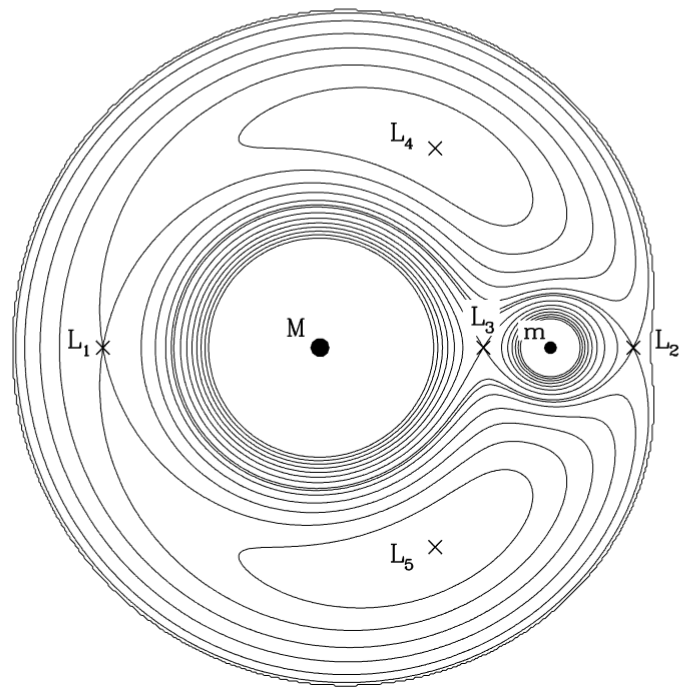
\includegraphics[width=0.5\textwidth]{assets/tides.png}
    \caption{Contours of equal effective potential $\Phi_{\mathrm{eff}}$ for two point masses in a circular orbit, with mass ratio $m/M = 1/9$. The locations L1, \ldots, L5 are the Lagrange points. L4 and L5 form equilateral triangles with the two masses. \cite{binney}}
\end{figure}